\section{Development-split results}\label{sec:resDEV}
Everything in this section uses DEV scenes only and was fixed before any test image was generated. It is exploratory; its role is to set constants and to decide, through pre-declared gates, which claims the test split can carry.

\paragraph{An estimator error found and corrected before the test split.} The chance-agreement term $A0$ had first been computed from every core image of a scene, including paraphrases, counterfactual variants and other guidance scales, instead of only independent seeds of the branches' own base prompt as specified. This lowers $A0$ and biases every $C(t)$ upwards. The code was corrected, a regression test added, and the DEV constants were recomputed from the stored judgements; both versions are archived. All DEV numbers below use the corrected estimator.

\paragraph{Persistence curves.} Figure~\ref{fig:devcurves} shows $C(t)$ on \devScenesHA{} DEV scenes. Presence crosses $0.5$ near $t_{50}=\tPres$ steps (D8); colour binding given presence is already above $0.5$ at the first grid step (left-censored, $t_{50}\le\tBind$), and count is latest ($\tCount$). With both restart probes the binding-minus-presence difference is negative but its interval includes zero: D8 $\Delta t_{50}=\dtDeight$ $[\dtDeightLo,\dtDeightHi]$, ER30 $\dtErThirty$ $[\dtErThirtyLo,\dtErThirtyHi]$ (Table~\ref{tab:dev-t50}). Left-censoring means DEV cannot place binding relative to presence; and the binding judge missed the audit criterion.
\begin{figure}[t]\centering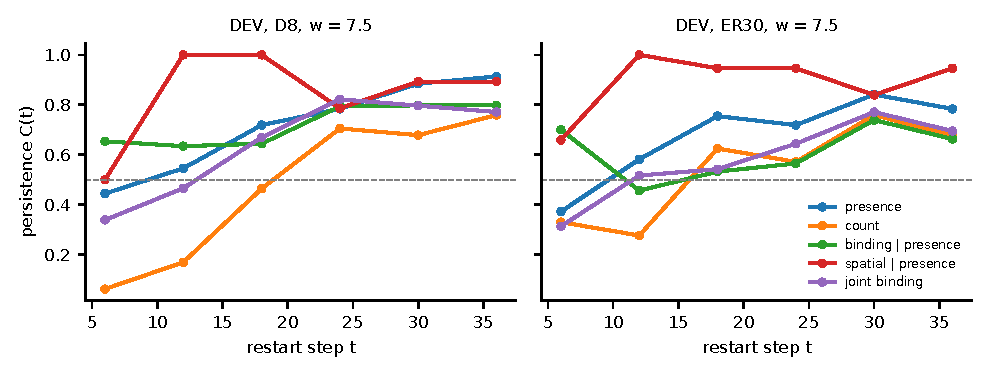
\includegraphics[width=\linewidth]{figures/fig_dev_curves.pdf}
\caption{DEV restart persistence $C(t)$ at $w=7.5$ for the fixed-jump (D8) and equal-ratio (ER30) probes (corrected estimator; exploratory). Dashed line: $C=0.5$.}\label{fig:devcurves}\end{figure}
\begin{table}[t]\centering\small
\caption{DEV persistence steps $t_{50}$ at $w=7.5$ (EXPLORATORY; 163 scenes). $^{\dagger}$left-censored: already above 0.5 at the first grid step.}\label{tab:dev-t50}
\begin{tabular}{lrr}
\toprule
Kind & D8 & ER30 \\
\midrule
presence & 9.3 & 9.7 \\
count & 18.9 & 15.8 \\
binding $\mid$ presence & 6.0$^{\dagger}$ & 6.0$^{\dagger}$ \\
spatial $\mid$ presence & 6.0 & 6.0$^{\dagger}$ \\
joint binding & 13.0 & 11.5 \\
$\Delta t_{50}$ (binding $-$ presence) & -3.29 [-7.56, 8.32] & -3.66 [-6.83, 6.77] \\
\bottomrule
\end{tabular}
\end{table}


\paragraph{Gates.} Table~\ref{tab:dev-gates} lists every pre-declared DEV gate. The HA precision gate failed (half-width \haHalfwidth{} steps against a limit of 4), so HA is exploratory on the test split by the pre-declared rule. The full-resample control failed (maximum $|C|=\fullMaxC$ against $0.15$): the statistic is a maximum over 30 cells, several resting on fewer than ten scenes, so even exactly independent outcomes rarely meet it at this sample size; but presence, the best-supported cell, shows a consistent offset of about $+0.16$ that sampling error does not explain and for which no cause was found in the code. We report it as an open validity concern for the restart estimator. Both HD presence gates passed (\hdPresTwo{} and \hdPresFifteen{} scenes).
\begin{table}[t]\centering\small
\caption{DEV gates (corrected estimator). Failed gates are reported as failed; HA is therefore exploratory.}\label{tab:dev-gates}
\begin{tabular}{llrl}
\toprule
Gate & Criterion & DEV value & Result \\
\midrule
HA precision & CI half-width $\le 4$ steps & 7.94 & failed \\
Full-resample control & $\max|C| \le 0.15$ & 0.57 & failed \\
HD presence, $w=2$ & $\ge 40$ scenes & 45 & passed \\
HD presence, $w=15$ & $\ge 40$ scenes & 59 & passed \\
CAG quality (HPS v2), $w_{lo}=1$ & mean drop $\le 0.5$ & -0.52 & failed \\
CAG quality (HPS v2), $w_{lo}=3$ & mean drop $\le 0.5$ & -0.26 & passed \\
\bottomrule
\end{tabular}
\end{table}


\paragraph{CAG quality guard.} HPS~v2 scored the \hpsPairs{} DEV guard images per $w_{lo}$ against their constant-CFG partners (same prompt and seed). With $w_{lo}=1$ the mean change was \hpsOne{} HPS points (95\% interval \hpsOneLo{} to \hpsOneHi), a drop just beyond the pre-declared $0.5$; with $w_{lo}=3$ it was \hpsThree{} (\hpsThreeLo{} to \hpsThreeHi). By the pre-declared rule $w_{lo}=3$ was adopted before the test split (Figure~\ref{fig:hps}). The switch steps derived from DEV are $s^\star=12$ for prompts whose latest type is presence, binding or spatial relation and $s^\star=21$ for prompts with counts (global $s^\star=\sStarGlobal$).
\begin{figure}[t]\centering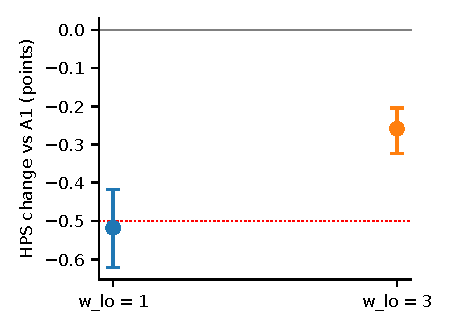
\includegraphics[width=0.45\linewidth]{figures/fig_hps_guard.pdf}
\caption{DEV CAG quality guard: mean HPS~v2 change of CAG images relative to constant CFG~7.5 (95\% scene-bootstrap intervals). Dotted line: pre-declared limit $-0.5$.}\label{fig:hps}\end{figure}
